\documentclass[10pt]{beamer}
%put handout in option above to disable the animation itemize/pause

\usepackage{xeCJK}
\setCJKmainfont{IPAMincho}
\setCJKsansfont{IPAGothic}
\setCJKmonofont{IPAGothic}

\usepackage{natbib}
\usepackage{hyperref}
\usepackage{graphicx}
\usepackage {mathtools}
\usepackage{forloop}
\usepackage{xcolor}

\usetheme{CambridgeUS}
\usecolortheme{dolphin}

% set colors
\definecolor{ehimeColor}{RGB}{248, 181, 0} %yellowis
\definecolor{ehimeColor2}{RGB}{55, 46, 42}
\definecolor{ehimeColor3}{RGB}{200, 184, 20}

\setbeamercolor{block title}{bg=ehimeColor,fg=black}
\setbeamercolor{block body}{bg=ehimeColor!20,fg=black}
\setbeamercolor{block title alerted}{bg=black, fg=ehimeColor}
\setbeamercolor{block body alerted}{bg=black!20, fg=black}

\setbeamercolor*{block title example}{bg=ehimeColor, fg = black}
\setbeamercolor*{block body example}{bg=ehimeColor!20, fg = black}
%\usebeamercolor[ehimeColor]{block title alerted}
\setbeamercolor*{palette primary}{bg=ehimeColor}
\setbeamercolor*{palette secondary}{bg=ehimeColor, fg = white}
\setbeamercolor*{palette tertiary}{bg=ehimeColor, fg = white}
\setbeamercolor*{titlelike}{fg=ehimeColor}
\setbeamercolor*{title}{bg=ehimeColor}
\setbeamercolor*{item}{fg=ehimeColor}
\setbeamercolor*{caption name}{fg=ehimeColor}
\usefonttheme{professionalfonts}

%------------------------------------------------------------
\titlegraphic{
\includegraphics[height=1.5cm]{ehime.png}} 

\setbeamerfont{title}{size=\large}
\setbeamerfont{subtitle}{size=\small}
\setbeamerfont{author}{size=\small}
\setbeamerfont{date}{size=\small}
\setbeamerfont{institute}{size=\small}


\title[Hamming(7,4)-Code]{Hamming(7,4)-Code}
%\subtitle{ Your Subtitle is Here}

\author[Arif Nurwahid]{Arif Nurwahid\inst{1}\\  source: \href{https://arif.page/hc}{arif.page/hc} | email: \href{mailto:me@arif.page}{me@arif.page}}%%authors

\institute[Ehime University]{Graduate School of Science and Engineering, Ehime University\inst{1}}

\date[\textcolor{ehimeColor2}{Mathematical Science, 2022}]
{Presentation Seminar on Mathematical Sciences\\
Nov 2, 2022}

%------------------------------------------------------------
%This block of commands puts the table of contents at the 
%beginning of each section and highlights the current section:
%\AtBeginSection[]
%{
%  \begin{frame}
%    \frametitle{Contents}
%    \tableofcontents[currentsection]
%  \end{frame}
%}
\AtBeginSection[]{
  \begin{frame}
  \vfill
  \centering
  \begin{beamercolorbox}[sep=8pt,center,shadow=true,rounded=true]{title}
    \usebeamerfont{title}\insertsectionhead\par%
  \end{beamercolorbox}
  \vfill
  \end{frame}
}
%------------------------------------------------------------
\begin{document}
%The next statement creates the title page.
\frame{\titlepage}
\begin{frame}
\frametitle{Table of Contents}
\tableofcontents
\end{frame}

%------------------------------------------------------------
\section{Introduction}
\begin{frame}{Introduction}
\frametitle{Introduction}
    \begin{block}{Question }
    Could you please raise your hand if you never heard about Hamming Code?
    \end{block}
    
    \begin{block}{質問 }
    ハミング コードについて聞いたことがない場合は、手を挙げていただけますか?
    \end{block}
\end{frame}

% -- Game Started - %
\section{Let's Play a Game}
\begin{frame}{Let's Play a Game}
\frametitle{Let's Play a Game (Rules)}
	\begin{enumerate}
		\item Please Pick a positive integer from 1 to 15
		\pause
		\item I will give you 7 questions. You can answer either YES or NO each question.
		\pause
		\item Here is the fun thing. You may \textbf{lie at most one time} when answering all questions in total.
	\end{enumerate}
\end{frame}

\newcounter{x}
\forloop{x}{1}{\value{x}<8}{
    \begin{frame}{Question \arabic{x}}
        \frametitle{Question \arabic{x}: : Do you see your chosen number?}
            \begin{figure}
                \includegraphics[width=0.8\textwidth]{question/Q\arabic{x}.png}
                \caption{List \arabic{x}}
            \end{figure}
    \end{frame}
}

\begin{frame}{Moment of Truth}
\frametitle{Result}
    \centering
	\Huge{Moment of Truth!}
\end{frame}

\begin{frame}{Try by Yourself}
\frametitle{Try by Yourself by adding this \textbf{Line Account}}
    \begin{figure}
        
\includegraphics[width=0.5\textwidth]{mathemagics.png}
        \caption{\textbf{Mathemagics} Line ID: \textbf{@025rlikw}}
    \end{figure}
\end{frame}

% -- Hamming Codes -- %
\section{Hamming(7,4) Codes}
\begin{frame}{Hamming(7,4) Codes}
    \begin{block}{What is Hamming(7,4) Codes?}
        \pause
        In coding theory, \textbf{Hamming(7,4)} is a \underline{linear error-correcting code} that encodes four bits of data into seven bits by adding three parity bits.
    \end{block}
\end{frame}

% -- Digital Communication Channel -- %
\section{Digital Communication Channel}
\begin{frame}{Digital Communication Channel}
    \begin{figure}
        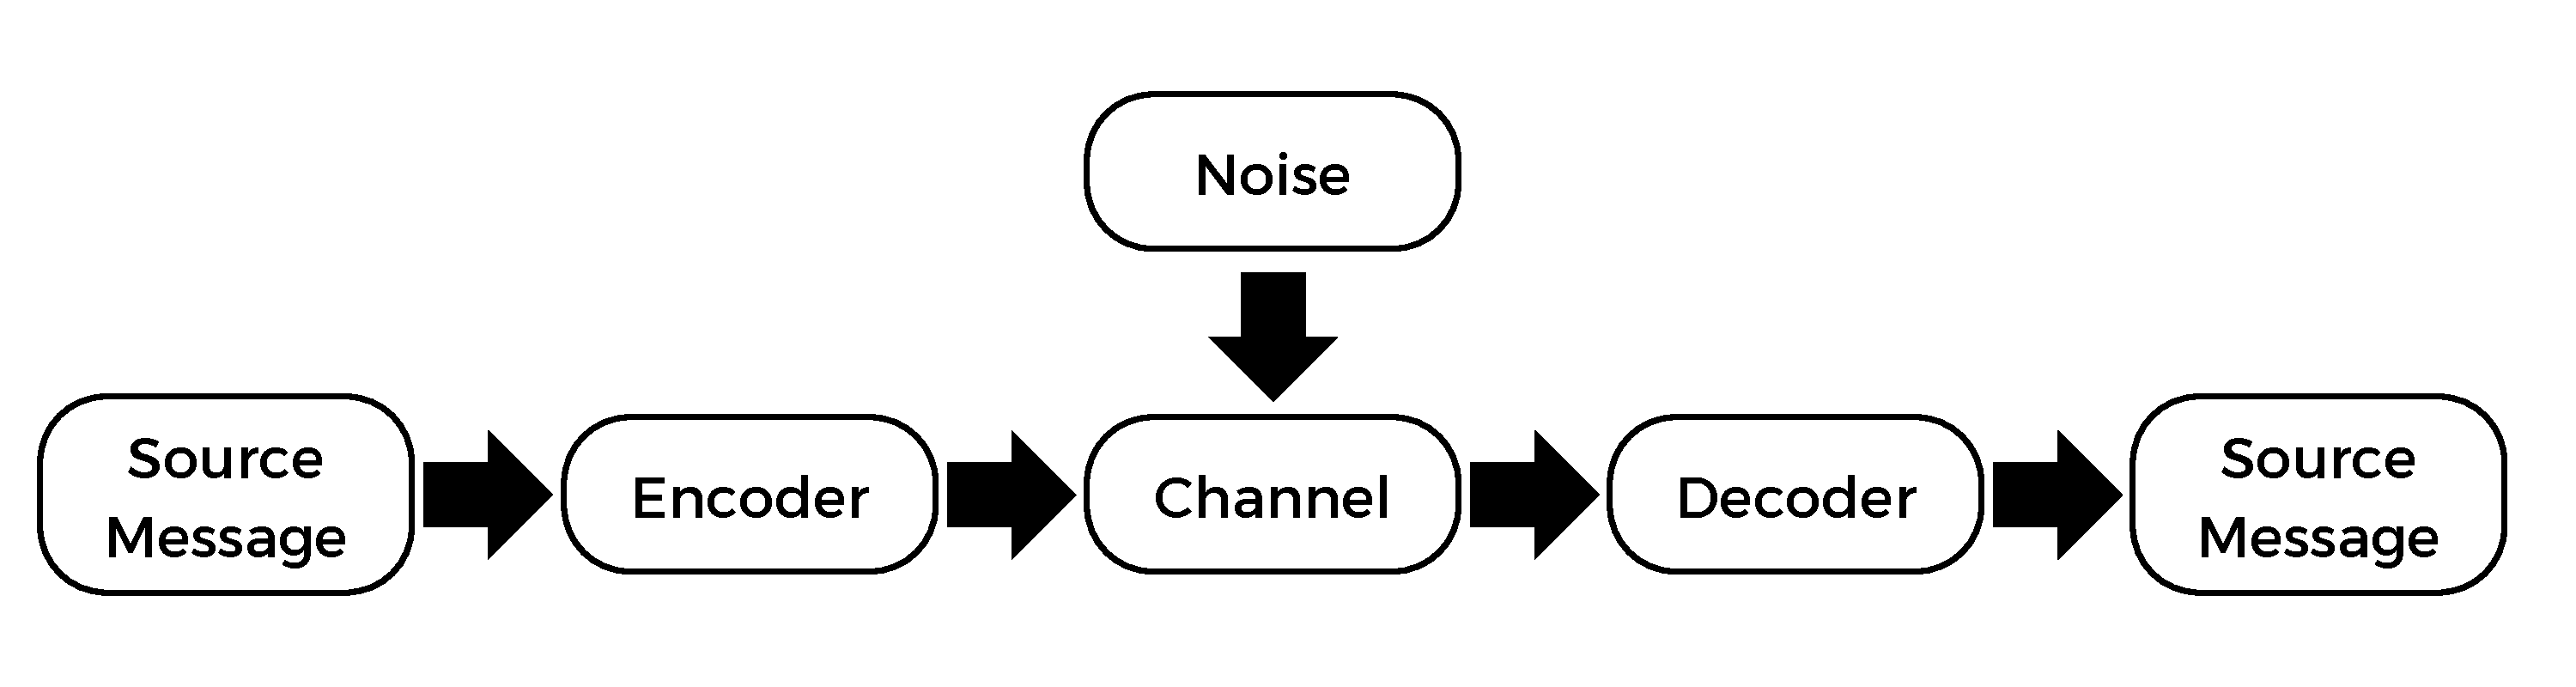
\includegraphics[width=\textwidth]{channel.pdf}
        \caption{Flow of Digital Communication Channel}
    \end{figure}
\end{frame}

\begin{frame}{Digital Communication Channel with Example}
    \begin{figure}
        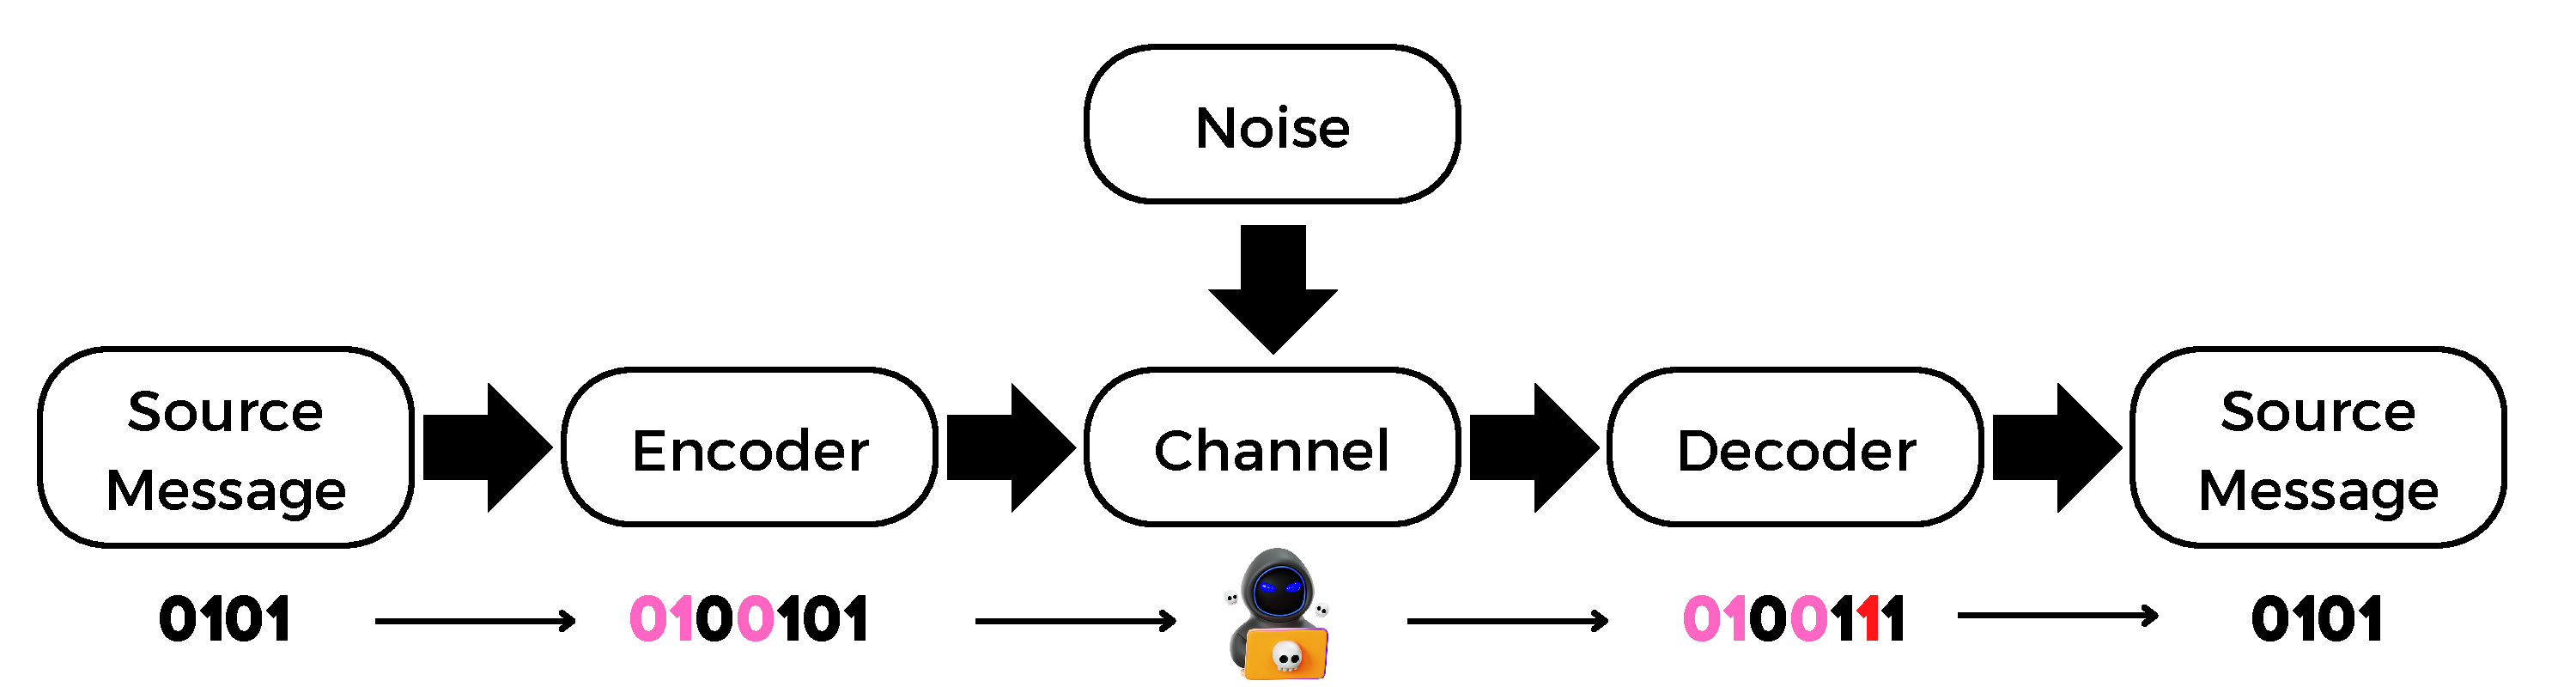
\includegraphics[width=\textwidth]{channel_e.pdf}
        \caption{Flow of Digital Communication Channel with Example}
    \end{figure}
\end{frame}

% -- Digital Communication Channel -- %
\section{Generator Matrix and Parity-check Matrix}
\begin{frame}{Generator Matrix and Parity-check Matrix}
    \begin{columns}
        \column{0.4\textwidth}
            \begin{align*}
                G^T := 
                \begin{pmatrix}
                1&1&0&1\\
                1&0&1&1\\
                1&0&0&0\\
                0&1&1&1\\
                0&1&0&0\\
                0&0&1&0\\
                0&0&0&1
                \end{pmatrix}
            \end{align*}
            the code generator matrix G
            
        \column{0.4\textwidth}
            \begin{align*}
                H := 
                \begin{pmatrix}
                1&0&1&0&1&0&1\\
                0&1&1&0&0&1&1\\
                0&0&0&1&1&1&1
                \end{pmatrix}
            \end{align*}
            the parity-check matrix H
    \end{columns}
\end{frame}

% -- example -- %
\section{Example}
\begin{frame}{Example}
    Suppose we want to transmit this data $(0111)$ over a noisy communications channel (specifically, a binary symmetric channel). Let's call it as vector $p$. Then,
    \begin{align*}
        x=G^T p = 
        \begin{pmatrix}
        1&1&0&1\\
        1&0&1&1\\
        1&0&0&0\\
        0&1&1&1\\
        0&1&0&0\\
        0&0&1&0\\
        0&0&0&1
        \end{pmatrix}
        \begin{pmatrix}
        0\\
        1\\
        1\\
        1
        \end{pmatrix}
        =
        \begin{pmatrix}
        2\\
        2\\
        0\\
        3\\
        1\\
        1\\
        1
        \end{pmatrix}
        =
        \begin{pmatrix}
        0\\
        0\\
        0\\
        1\\
        1\\
        1\\
        1
        \end{pmatrix}
    \end{align*}
This means that (0001111) would be transmitted instead of transmitting (0111).

For example, suppose a bit error occurs on bit 6 while transmitted, it turns to be (00011\textcolor{red}{0}1) as vector $r$.
\end{frame}



\begin{frame}{Example (cont.)}
     Let's do the parity-check,
    \begin{align*}
        z = H r = 
        \begin{pmatrix}
        1&0&1&0&1&0&1\\
        0&1&1&0&0&1&1\\
        0&0&0&1&1&1&1
        \end{pmatrix}
        \begin{pmatrix}
        0\\
        0\\
        0\\
        1\\
        1\\
        0\\
        1
        \end{pmatrix}
        =
        \begin{pmatrix}
        2\\
        1\\
        3
        \end{pmatrix}
        =
        \begin{pmatrix}
        0\\
        1\\
        1
        \end{pmatrix}
    \end{align*}
This means that error occurred on bit $(110)_2$, which is bit 6.
\end{frame}
% -------------------------


\section*{Acknowledgement}  
\begin{frame}
\textcolor{ehimeColor}{\Huge{\centerline{Thank You!}}}
\end{frame}

\end{document}



